%\documentclass[12pt,oneside]{book}

%% Маргине, проред и тако то
%\usepackage[a4paper, margin=30mm]{geometry}
%\renewcommand{\baselinestretch}{1.5}

%% Фонтови, енкодинг
%\usepackage[]{mathtext}
%\usepackage[T2A, TS1]{fontenc}
%\usepackage[utf8]{inputenc}
%\usepackage[english, russian, serbianc]{babel}
%%\usepackage[russian]{babel}
%\usepackage{babelbib}
%\setbtxfallbacklanguage{english}

%\usepackage{graphicx}
%\DeclareGraphicsExtensions{.pdf,.png,.jpg}
%\usepackage{tikz}

%\usepackage[cmex10]{amsmath}
%\usepackage{amssymb}

%\usepackage[caption=false,font=footnotesize]{subfig}
%\renewcommand{\thesubfigure}{\asbuk{subfigure}}

%\usepackage{siunitx}
%\sisetup{detect-all = true,
%range-phrase = --,
%range-units = single,
%output-decimal-marker = {,}}
%\usepackage{physics}
%\usepackage{nicefrac}
%\usepackage[siunitx]{circuitikz}

%%\usepackage[usenames,dvipsnames,svgnames,table]{xcolor}
%%\usepackage{soul}
%%%\definecolor{lightblue}{rgb}{.90,.95,1}
%%\colorlet{lightblue}{cyan!50}
%%\sethlcolor{lightblue}

%%\usepackage[nomarkers]{endfloat}%notablist,nofiglist ili nolists

%\usepackage[]{foreign}

%\title{АСИМЕТРИЧНИ РЕЗОНАТОРИ КАО ЕЛЕМЕНТИ ЈЕДИНИЧНИХ ЋЕЛИЈА ЈЕДНОДИМЕНЗИОНАЛНИХ МЕТАМАТЕРИЈАЛА}
%\date{\today}
%\author{Војислав Милошевић}

%\begin{document}

\chapter{Увод}

%\tableofcontents

\section{Основни појмови}

Метаматеријали се могу дефинисати као вештачке композитне структуре, које поседују необичне особине, које је тешко, или немогуће, наћи у природи~\cite{Sham:09}. Очигледно је оваква дефиниција веома општа, међутим, услед велике разноврсности у самој области, као и непостојања консензуса у литератури, тешко је дати прецизнију свеобухватну дефиницију. У наставку ће бити дат преглед области...% хм... некако би требало ово мало преправити

Особине метаматеријала од интереса готово искључиво су везане за њихову интеракцију са различитим типовима таласа. Најчешће, у питању су електромагнетни (ЕМ) таласи, у ком случају се говори о ЕМ метаматеријалима, мада постоје и други типови (нпр. акустички). У овој тези ће се говорити искључиво о ЕМ метаматеријалима, што се у даљем тексту неће посебно наглашавати.

Метаматеријали се обично реализују као периодичне структуре са резонантним елементима, при чему периодичност може бити у једној, две или три димензије. Претпоставка је да је период, $d$, много мањи од таласне дужине, $\lambda$, у опсегу од интереса (обично у околини резонансе елемената), тако да се метаматеријал понаша као континуална средина~\cite{landau1982}. У том случају се може извршити хомогенизација Максвелових једначина, при чему се материјал описује \emph{ефективним параметрима}, као што су диелектричка пермитивност, $\varepsilon$, магнетна пермеабилност, $\mu$. Разлика у односу на фотонске кристале, који су такође периодичне структуре, дефинише се преко односа $\frac{d}{\lambda}$; уколико је он мањи од $\frac{1}{2}$, што одговара првој Браговој резонанси, ради се о режиму метаматеријала. За већину метаматеријала приказаних у литератури овај однос је приближно око $\frac{1}{4}$. С обзиром да је овај однос много већи него што је обично случај за природне материјале, хомогенизација метаматеријала је предмет одређених контроверзи~\cite{simovski}.

Микроталасна техника се бави пројектовањем кола, компонената и система који раде на учестаностима условно од \SI{300}{\mega\hertz} до \SI{300}{\giga\hertz} (односно таласне дужине од \SI{1}{\meter} до \SI{1}{\milli\meter}). Прецизнији опис је да се ради о колима чије димензије су упоредиве са таласном дужином сигнала, што има битне последице на начин рада и пројектовање. На пример, за пренос сигнала морају се користити водови или таласоводи, чије особине битно утичу на остатак кола, за разлику од нижих учестаности, где се сигнал преноси било каквим електричним контактом, чији утицај се може занемарити. Најважније примене микроталасне технике су најпре радарски системи и телекомуникације, који раде на овим учестаностима због широког опсега и повољних услова простирања, и довољно мале таласне дужине да се могу направити усмерене антене. Такође, многе атомске и молекуларне резонансе од интереса налазе у микроталасном опсегу, због чега постоје примене у радио-астрономији, медицини, даљинској детекцији (\foreign{remote sensing})~\cite{djordjevic2005mikrotalasna,pozar2009microwave}.  \cite{markes_knjiga}

\section{Особине средине са истовремено негативним параметрима $\varepsilon$ и $\mu$}
\subsection{Простирање таласа}

Очекивано је да реални делови пермитивности, $\varepsilon$, и пермеабилности, $\mu$, буду позитивни – ово произилази из једноставне чињенице да се елементарна наелектрисања и магнетни моменти у материјалу оријентишу у смеру спољашњег поља. Ипак, ако се посматрају временски променљива поља, мора се узети у обзир дисперзија параметара, $\varepsilon(\omega)$ и $\mu(\omega)$; и могуће је да постоје негативне вредности на одређеним фреквенцијама. Многи материјали у природи испољавају $\varepsilon < 0$, нпр. плазма испод Друдеове учестаности. Материјали са $\mu<0$ су ретки, али ово својство испољавају нпр. ферити на микроталасним учестаностима. Ипак, све до недавно нису били познати материјали код којих би истовремено важило $\varepsilon,\mu < 0$.

У свом познатом раду, Веселаго је хипотетички разматрао постојање таквог материјала~\cite{veselago_cir}. У изотропној средини, из Максвелових једначина може се извести скаларни облик таласне једначине:
\begin{equation}
    \left( \nabla^2 - \frac{n^2}{c^2}\frac{\partial}{\partial t} \right) \psi = 0.
    \label{uvod:skalarwave}
\end{equation}
где је $n^2 = \varepsilon\mu$, а $c$ је брзина светлости. Истовремена промена знака $\varepsilon$ и $\mu$ неће ништа променити у (\ref{uvod:skalarwave}), па се може поставити питање какав би био утицај ове промене. Веселаго предвиђа три могућа одговора:
\begin{itemize}
    \item истовремена промена знака $\varepsilon$ и $\mu$ никако не утиче на особине средине;
    \item постоје физички закони који забрањују истовремено негативне вредности $\varepsilon$ и $\mu$;
    \item материјали са негативним $\varepsilon$ и $\mu$ имају другачије особине од оних са позитивним.
\end{itemize}
Показује се да је последњи од ових одговора тачан~\cite{veselago_cir}. Да би се уверили у то, потребно је размотрити полазне Максвелове једначине:
\begin{align}
    \nabla\times \vec{E} & = -j\omega\mu \vec{H} \\
    \nabla\times \vec{H} & =  j\omega\varepsilon \vec{E} .
\end{align}
За равански талас, ове једначине се своде на:
\begin{align}
    \vec{k} \times \vec{E} & =  \omega\mu\vec{H} \\
    \vec{k} \times \vec{H} & = -\omega\varepsilon\vec{E} ,
\end{align}
где је $\vec{k}$ таласни вектор. Из ових израза види се да $\vec{E}$, $\vec{H}$ и $\vec{k}$ чине скуп ортогоналних вектора који су повезани правилом десне руке. Промена знака $\varepsilon$ и $\mu$ мења оријентацију, па у том случају ови вектори чине триплет повезан правилом леве руке (илустрација?). Због тога се овакви материјали називају „леворуки`` (\foreign{left-handed, LH}). Испоставља се да ово својство има суштинске последице на простирање таласа. Наиме, ако размотримо Поинтингов вектор, који представља простирање енергије:
\begin{equation}
    \vec{S} = \vec{E} \times \vec{H},
\end{equation}
се не мења као последица промене знака $\varepsilon$ и $\mu$, због чега су $\vec{S}$ и $\vec{k}$ антипаралелни. Другим речима, енергија и таласни фронт се простиру у супротним смеровима у таквој средини (\foreign{backward-wave}).

губици...

густина енергије и групна брзина...

\subsection{Негативна рефракција}

\begin{figure}[h]
    \centering
    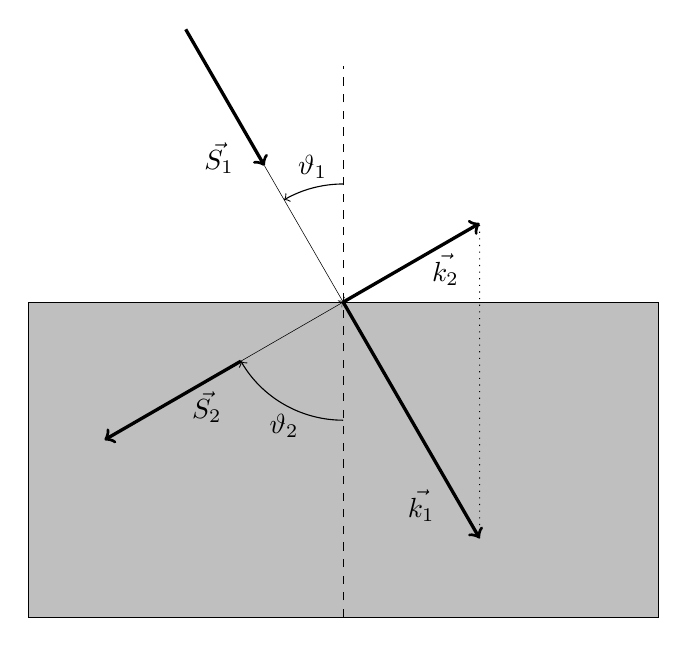
\begin{tikzpicture}
        \draw[fill=lightgray] (-4,-4) rectangle (4,0);
        \draw[dashed] (0,-4) -- (0,3);
        \draw[->, very thick] (0,0) -- (30:2cm)  node[near end, below] {$\vec{k_2}$};% -- ++(0,-5);
        \draw[->, very thick] (0,0) -- (-60:3.464cm) node[near end, below left] {$\vec{k_1}$};
        \draw[->, very thick] (120:4cm) -- (120:2cm) node[near end, below left] {$\vec{S_1}$};
        \draw[->, very thin] (120:2cm) -- (0,0);% node[near end, below left] {$\vec{k_1}$};
        \draw[->] (0,1.5) arc (90:120:1.5cm) node[midway, above] {$\vartheta_1$};
        \draw[<-, very thick] (-150:3.5cm) -- (-150:1.5cm) node[near end, below ] {$\vec{S_2}$};
        \draw[->, very thin] (-150:2cm) -- (0,0);% node[near end, below left] {$\vec{k_1}$};
        \draw[->] (0,-1.5) arc (-90:-150:1.5cm) node[midway, below] {$\vartheta_2$};
        \draw[dotted] (-60:3.464cm) -- (30:2cm);
        
    \end{tikzpicture}   
    \caption{Преламање таласа на граници између обичне (1) и „леворуке`` средине (2).}
    \label{uvod:negrefr}
\end{figure}
Замислимо талас, инцидентан на граничну површину која раздваја „леворуку`` и обичну средину ($\varepsilon,\mu > 0$), као што је приказано на сл.~\ref{uvod:negrefr}. Гранични услови захтевају континуитет тангенцијане компоненте таласног вектора, из чега следи да упадни угао и угао преламања имају супротне знаке. Ако узмемо у обзир Снелов закон:
\begin{equation}
    \frac{\sin{\vartheta_1}}{\sin{\vartheta_2}} = \frac{n_2}{n_1}
\end{equation}
следи да је индекс преламања у „леворукој`` средини негативан, $n_2<0$. Због тога се често користи термин средине са негативним индексом (\foreign{negative refractive index media}).

Негативни индекс доводи до инверзије многих физичких закона, па се тако конвексна сочива понашају као конкавна и обрнуто. Такође долази до инверзије Доплеровог ефекта, зрачења Черенкова „уназад``, негативног Гус-Хенхеновог помераја~\cite{markes_knjiga}.

\subsection{Савршено сочиво}

\begin{figure}[h]
    \centering
    \begin{tikzpicture}
        \usetikzlibrary{positioning,calc,intersections,decorations.markings}
        \draw[fill=lightgray] (-2,-4) rectangle (2,4);
        %\draw[step=1.0,black,thin] (-5,-5) grid (5,5);
        \path[name path=levo]  (-2,-4) -- (-2,4);
        \path[name path=desno] (2,-4)  -- (2,4);
        \draw[dashed,name path=horiz] (-4.7,0)  -- (5,0);
        \node at (0,3) {$n=-1$};
        \coordinate (iz) at (-3.5,0);

        \begin{scope}[thick, red, decoration={
    markings,
    mark=at position 0.5 with {\arrow{>}}}]
            
        \path[name path=zr1]  (iz) -- ++(20:5cm);
        \path [name intersections={of=zr1 and levo, by={pr1a}}];
        \draw[postaction={decorate}] (iz) -- (pr1a);
        \path[name path global=zr1b]  (pr1a) -- ++(-20:5cm);
        \path [name intersections={of=zr1b and desno, by={pr1b}}];
        \draw[postaction={decorate}] (pr1a) -- (pr1b);
        \path[name path=zr1c]  (pr1b) -- ++(20:5cm);
        \path [name intersections={of=zr1c and horiz, by={pr1c}}];
        \draw[postaction={decorate}] (pr1b) -- (pr1c);

        \end{scope}

        \begin{scope}[thick, blue, decoration={
                markings,
            mark=at position 0.5 with {\arrow{>}}}]
            
        \path[name path=zr2]  (iz) -- ++(-45:5cm);
        \path [name intersections={of=zr2 and levo, by={pr2a}}];
        \draw[postaction={decorate}] (iz) -- (pr2a);
        \path[name path global=zr2b]  (pr2a) -- ++(45:7cm);
        \path [name intersections={of=zr2b and desno, by={pr2b}}];
        \draw[postaction={decorate}] (pr2a) -- (pr2b);
        \path[name path=zr2c]  (pr2b) -- ++(-45:5cm);
        \path [name intersections={of=zr2c and horiz, by={pr2c}}];
        \draw[postaction={decorate}] (pr2b) -- (pr2c);

        \end{scope}

        \draw[densely dashed] (iz) -- ++(0,-2) ++(8,0) -- ++(0,2);
        \draw[<->] (iz) ++(0,-1.8) -- ++(8,0) node[midway, below] {$2d$};
        \draw[<->] (-2,-3) -- ++(4,0) node[midway, below] {$d$};

        \path [name intersections={of=zr1b and zr2b, by={f1}}];
        \filldraw (f1) circle (2pt) node[below] {$F_1$};
        \filldraw (iz) circle (2pt) node[below left] {извор}
            ++(8,0) circle (2pt) node[below right] {$F_2$};
    \end{tikzpicture}
    \caption{Сочиво...}
    \label{uvod:ssocivo}
\end{figure}
Једна од најзанимљивијих особина средине са негативним индексом се састоји у следећем. Претпоставимо плочу, дебљине $d$, са индексом преламања $n=-1$, која се налази у вакууму (сл.~\ref{uvod:ssocivo}). На граничним површинама, упадни зраци се преламају под истим углом под којим долазе, симетрично у односу на нормалу, $\vartheta_1 = \vartheta_2$. Уколико се тачкасти извор налази на растојању $a$ од ивице, при чему је $a<d/2$, показује се да се оваква плоча понаша као сочиво, са две тачке фокуса -- једна у унутрашњости плоче, а друга на растојању $2d$ од извора~\cite{veselago_cir}.

Како би се детаљније испитала способност плоче материјала са негативним индексом да се понаша као сочиво, није довољна апроксимација геометријске оптике, већ је потребно размотрити понашање електромагнетних таласа. Најзанимљивији случај је материјал са $\nicefrac{\varepsilon}{\varepsilon_0}\to 1$ и $\nicefrac{\mu}{\mu_0}\to 1$. Пендри је показао, у свом познатом раду, да је овакво сочиво у стању да реконструише комплетно поље из равни извора на растојању $2d$~\cite{pendry3}. На овај начин се формира слика која превазилази дифракциони лимит, због чега је овакво сочиво добило епитет „савршено``. Појава се може тумачити помоћу експанзије поља у просторне хармонике. Показује се да је материјал са негативним индексом у стању да пренесе не само пропагационе модове, као обично сочиво, већ и еванесцентне~\cite{markes_knjiga}. У пракси се морају размотрити губици, који онемогућавају постизање идеалних резултата, али у литератури се могу наћи извештаји о оствареној резолуцији испод дифракционог лимита~\cite{grbic2004overcoming}.

\subsection{Реализација}

\begin{figure}[h]
    \centering
    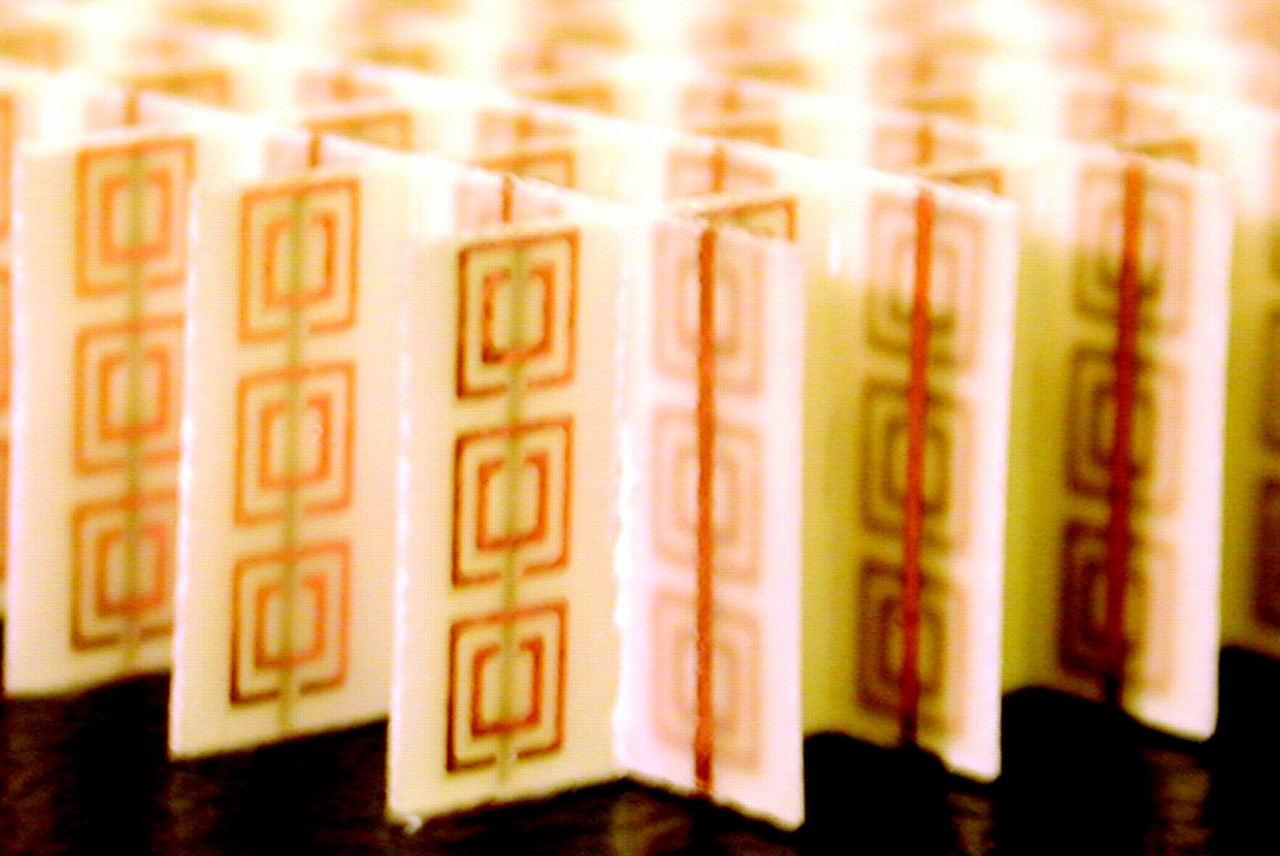
\includegraphics[width=0.8\linewidth]{sl_uvod/mm_smit.jpg}
    \caption{Експериментална реализација метаматеријала са негативними индексом~\cite{smith:00}.}
    \label{uvod:mm_smit}
\end{figure}
Прошло је више од тридесет година од Веселагове теоријске спекулације до реализације негативног индекса помоћу метаматеријала. Историјски, коришћење периодичних структура за синтезу диелектричне константе у микроталасној техници датира из педесетих година прошлог века, када су биле познате под термином „вештачки диелектрици`` (\foreign{artificial dielectric})~\cite{rotman1962plasma}. Пендри је предложио коришћење резонатора у облику прстена са процепом, тзв. сплит ринг резонатор, СРР (\foreign{split-ring, SRR}) за синтезу негативне пермеабилности~\cite{pendri:99}. Комбинацијом ова два приступа, фабриковани су метаматеријали који испољавају негативни индекс преламања у микроталасном опсегу~\cite{smith:00}.

Метаматеријал $<=>$ негативни индекс? Можда нешто рећи о томе докле су стигли са свим будалаштинама?

\section{Метаматеријали и водови}

\subsection{Дуални вод}

\begin{figure}[h]
    \centering
    \subfloat[]{
    \begin{tikzpicture}[scale=0.9]
        \ctikzset{tripoles/mos style/arrows}
        \draw 
            (-2,0) to [short] ++(0.75,0)
            to [L=$L$] ++(2.5,0)
            to [short] ++(0.75,0)


            (-1.25,0) to [C=$C$] ++(0,-2)
            node [ground] {}

            (1.25,0) to [C=$C$]++(0,-2)
            node [ground] {}

            ;
        \draw[dashed]
            (-2,0) -- ++(-1,0)
            (2,0) -- ++(1,0)
            ;
        \draw[<->] (-1.25,1) -- (1.25,1) node[midway,above] {$l$};
        \draw[densely dashed] (-1.25,0) -- ++(0,1.2)
            (1.25,0) -- ++(0,1.2);


    \end{tikzpicture}\label{uvod:rhvod}}\hfil
    \subfloat[]{
    \begin{tikzpicture}[scale=0.9]
        \ctikzset{tripoles/mos style/arrows}
        \draw 
            (-2,0) to [short] ++(0.75,0)
            to [C=$C$] ++(2.5,0)
            to [short] ++(0.75,0)


            (-1.25,0) to [L=$L$] ++(0,-2)
            node [ground] {}

            (1.25,0) to [L=$L$]++(0,-2)
            node [ground] {}

            ;
        \draw[dashed]
            (-2,0) -- ++(-1,0)
            (2,0) -- ++(1,0)
            ;

        \draw[dashed]
            (-2,0) -- ++(-1,0)
            (2,0) -- ++(1,0)
            ;
        \draw[<->] (-1.25,1.2) -- (1.25,1.2) node[midway,above] {$l$};
        \draw[densely dashed] (-1.25,0) -- ++(0,1.4)
            (1.25,0) -- ++(0,1.4);
    \end{tikzpicture}\label{uvod:lhvod}}
    \caption{Елементарна ћелија, дужине $l$, обичног вода (а) и дуалног (б).}
    %\label{fig:}
\end{figure}
Паралелно са развојем тродимензионалних метаматеријала, појавио се алтернативни концепт за реализацију негативног индекса преламања, односно инверзних таласа, на бази теорије водова~\cite{bib2,bib4,bib3}. Наиме, постоји аналогија између Максвелових једначина и једначина телеграфичара за водове, где напон одговара електричном пољу, а струја магнетном. Елементарна секција вода испуњеног „нормалним`` диелектриком (са $n>0$) приказана је на сл.~\ref{uvod:rhvod}. Размотримо дуалну структуру, на којој су замењена места реактивних елемената (сл.~\ref{uvod:lhvod}). Применом теорије периодичних структура~\cite{pozar2009microwave}, можемо одредити фазну константу простирања, $\beta$, и Блохову импедансу, $Z_B$:
\begin{align}
    \cos{\beta l} & = 1 - \frac{\omega_c^2}{2\omega^2},\\%деф. дужину ћелије!!
    Z_b & = \sqrt{\frac{L}{C}\left(1-\frac{\omega_c^2}{\omega^2}\right)},
\end{align}
где је $\omega_c = \nicefrac{2}{\sqrt{LC}}$. Ако је ћелија много мања од таласне дужине, важи $\omega\ll\omega_c$. У том случају се горњи изрази могу апроксимирати као:
\begin{align}
    \beta l & = -\frac{\omega_c}{\omega},\\
    Z_B & = \sqrt{\frac{L}{C}} \equiv Z_C,
\end{align}
где је $Z_C$ карактеристична импеданса вода испуњеног обичним диелектриком. У овој апроксимацији се може показати да су параметри ефективног диелектрика, који би испуњавао овакав вод, негативни~\cite{markes_knjiga}.

Дисперзиони дијаграми...

\subsection{Композитни водови}

\begin{figure}[h]
    \centering
    \begin{tikzpicture}[scale=0.9]
        \ctikzset{tripoles/mos style/arrows}
        \draw 
            (-2,0) 
            to [L=$L_R$] ++(2.0,0)
            to [C=$C_L$] ++(2.0,0)


            (-2.0,0) -- ++(0,-1)
            -- ++(-1,0)
            to [C=$C_R$] ++(0,-2)
            -- ++(1,0)
            node [ground] {}

            (-2,-1)-- ++(1,0)
            to [L=$L_L$] ++(0,-2)
            -- ++(-1,0)


            (2.0,0) -- ++(0,-1)
            -- ++(-1,0)
            to [C=$C_R$] ++(0,-2)
            -- ++(1,0)
            node [ground] {}

            (2,-1)-- ++(1,0)
            to [L=$L_L$] ++(0,-2)
            -- ++(-1,0)

            (-2,0) -- ++(-1,0)
            (2,0) -- ++(1,0)

            ;

        \draw[dashed]
            (-3,0) -- ++(-1,0)
            (3,0) -- ++(1,0)
            ;

    \end{tikzpicture}
    \caption{Композитни вод.}
    \label{uvod:crlh}
\end{figure}
\begin{figure}[h]
    \centering
    \subfloat[]{\begin{tikzpicture}
        \draw[] (-3,3) -- (-3,-3) node[below] {$-\pi$}
            -- (0,-3) node[below] {$\beta l$}
            -- (3,-3) node[below] {$\pi$} -- ++(0,6);
        \draw[->] (0,-3) -- (0,3.2) node[right] {$\omega$};
        %\draw[scale=0.5,domain=-3:3,smooth,variable=\x,blue] plot ({\x},{\x*\x});
        %\draw[scale=0.5,domain=-3:3,smooth,variable=\y,red]  plot ({cos(\y)},{\y});
        %\draw[scale=0.5,domain=-3:3,smooth,variable=\y,red]  plot (\y,{cos(\y)});
        \draw [domain=-3:0, samples=50, blue] plot (\x,{-1.8+0.5*cos(pi*\x r/3)}) node[right] {$\omega_s$};
        \draw [domain=-3:0, xshift=3cm, samples=50, red] plot (\x,{1.2+1.1*cos(pi*\x r/3)});
        \draw[red] (0,0.0) node[left] {$\omega_p$};
    \end{tikzpicture}\label{uvod:d_nebalans} }\hfill
    \subfloat[]{\begin{tikzpicture}
        \draw[] (-3,3) -- (-3,-3) node[below] {$-\pi$}
            -- (0,-3) node[below] {$\beta l$}
            -- (3,-3) node[below] {$\pi$} -- ++(0,6);
        \draw[->] (0,-3) -- (0,3.2) node[right] {$\omega$};
        %\draw[scale=0.5,domain=-3:3,smooth,variable=\x,blue] plot ({\x},{\x*\x});
        %\draw[scale=0.5,domain=-3:3,smooth,variable=\y,red]  plot ({cos(\y)},{\y});
        %\draw[scale=0.5,domain=-3:3,smooth,variable=\y,red]  plot (\y,{cos(\y)});
        %\draw [domain=-3:0, samples=50, blue] plot (\x,{-1.8+0.5*cos(pi*\x r/3)}) node[right] {$\omega_s$};
        \draw [domain=-3:3, samples=50, olive] plot (\x,{1.6*sin(pi*\x r/6)});
        \draw[olive] (0,0.0) node[below right] {$\omega_0$};
    \end{tikzpicture}\label{uvod:d_balans} }
    \caption{Дисперзија фазне константе простирања на композитном воду.}
    %\label{fig:}
\end{figure}
Директна реализација дуалног вода са сл.~\ref{uvod:lhvod} у пракси била би могућа само на веома ниским учестаностима, када је могуће занемарити ефекте простирања. У микроталасном опсегу, неопходно је постојање обичног вода као носиоца простирања таласа, који се затим оптерећује реактивним елементима -- редним капацитивностима и паралелним индуктивностима. Допринос овог основног вода није могуће занемарити, одговарајућа еквивалентна шема јединичне ћелије представља комбинацију сл.~\ref{uvod:rhvod} и \ref{uvod:lhvod}, и приказана је на сл.~\ref{uvod:crlh}. У литератури су овакве структуре познате под називом \emph{композитни водови} (\foreign{composite right-/left-handed transmission line, CRLH TL}). Параметри дуалне структуре су $C_L$ и $L_L$, док $C_R$ и $L_R$ одговарају воду носиоцу. Применом теорије периодичних структура, добијају се следећи изрази за дисперзиону релацију:
\begin{align}
    \cos{\beta l} & = 1 - \frac{\omega^2}{2\omega_R^2}\left( 1 - \frac{\omega_s^2}{\omega^2} \right)\left( 1 - \frac{\omega_p^2}{\omega^2} \right),\label{uvod:beta_crlh} \\
    Z_B & = \sqrt{\frac{L_R}{C_R}\frac{1-\frac{\omega_s^2}{\omega^2}}{1-\frac{\omega_p^2}{\omega^2}} - \frac{L_R^2\omega^2}{4}\left( 1 - \frac{\omega_s^2}{\omega^2} \right)^2},
\end{align}
где су
\begin{align}
    \omega_R & = \frac{1}{\sqrt{L_R C_R} },\\
    \omega_L & = \frac{1}{\sqrt{L_L C_L} },
\end{align}
резонансе обичног и дуалног вода, респективно, и
\begin{align}
    \omega_s & = \frac{1}{\sqrt{L_R C_L} },\\
    \omega_p & = \frac{1}{\sqrt{L_L C_R} },
\end{align}
представљају резонантне фреквенције у редној и паралелној грани композитног вода.

%%%%%%%%%%%%%%%%%%%%%%%%%%%%%%%%%%%%%%%%%%%%%
%  коментар где је лефт, а где рајт хендид  %
%%%%%%%%%%%%%%%%%%%%%%%%%%%%%%%%%%%%%%%%%%%%%
Тражењем реалних решења (\ref{uvod:beta_crlh}) испоставља се да постоје две фреквентне зоне простирања, раздвојене процепом, као што је приказано на сл.~\ref{uvod:d_nebalans}. Границе процепа су одређене учестаностима $\omega_s$ и $\omega_p$, између којих не постоје реална решења за $\beta$. Уколико размотримо специјалан случај $\omega_s = \omega_p$, процеп неће постојати, и дисперзија добија изглед као на сл.~\ref{uvod:d_balans}. Овај случај у литератури је познат као \emph{балансни композитни вод}, и занимљив је за многе примене, зато што омогућава манипулацију са фазним померајем на воду, задржавајући стабилну карактеристичну импедансу.

\begin{figure}[h]
    \centering
    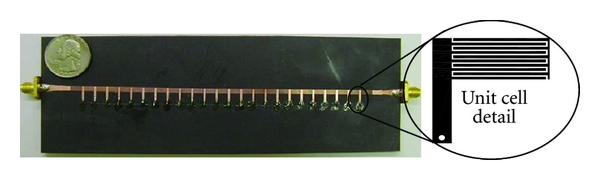
\includegraphics[width=1.0\linewidth]{sl_uvod/crlh_kalo.jpg}
    \caption{Пример композитног вода~\cite{caloz2005}.}
    \label{uvod:crlh_kalo} 
\end{figure}
Приликом реализације композитних структура, најпре је потребно одабрати основни вод – носилац. Иако је у принципу могуће користити било коју врсту вода, због лакоће фабрикације и интеграције најчешће се бирају планарни водови, као што су микрострип или копланарни таласовод. Затим се врши избор реактивних компоненти за реализацију дуалне структуре, за шта се могу користити готове компоненте са концентрисаним параметрима или дистрибуиране компоненте у техници водова. У првом случају су димензије реактивних елемената мање, па је самим могуће остварити већи опсег у коме се структура понаша као ефективно хомогена. С друге стране, вредности доступних реактанси су ограничене на оне које нуди произвођач, и интеграција са водом (најчешће лемљењем) компликује фабрикацију и уноси потенцијалне грешке. Дистрибуиране компоненте се лакше фабрикују, раде на вишим учестаностима, али потребно је водити рачуна о њиховој величини како би се добила ефективно хомогена структура.

Пример реализације композитног вода, са капацитивностима реализованим преко интердигиталних кондензатора, а индуктивностима помоћу уземљених огранака вода, дат је на сл.~\ref{uvod:crlh_kalo}. Овакве структуре су коришћене за бројне практичне апликације, које представљају унапређење у односу на раније познато стање, између осталих минијатуризоване делитеље/сабираче снаге~\cite{caloz2004novel}; подешавање импедансе у опсегу који је недоступан помоћу класичних водова~\cite{damm2007electrically}; антене са ,,цурећим`` таласом (leaky-wave), које се могу скенирати „уназад“~\cite{roig2013liquid}. Такође, концепт дуалног вода може се проширити у две димензије, за синтезу планарних метаматеријала~\cite{grbic2004overcoming,798001}.

\subsection{Резонантни приступ}%

Поступак синтезе дуалних водова, описан у претходној секцији, у литератури је познат под називом \emph{нерезонантни}, зато што се за постизање негативних вредности параметара користе реактивни елементи, који немају резонансе у опсегу од интереса. Могућ је и други приступ, \emph{резонантни}, где се водови и таласоводи периодично спрежу са подталасним резонаторима, као што су сплит ринг и сродне топологије. У том случају, еквивалентна шема ћелије биће нешто сложенија него на сл.~\ref{uvod:crlh}, али са веома сличним карактеристикама – такође испољава композитну природу, и поседује опсеге са негативним и нормалним параметрима~\cite{markes_knjiga}.

\begin{figure}[h]
    \centering
    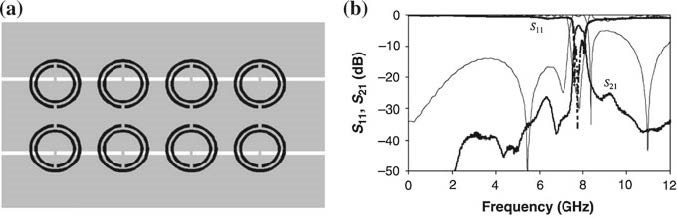
\includegraphics[width=1.0\linewidth]{sl_uvod/cpw.jpg}
    \caption{Резонантни „леворуки`` вод на бази копланарног таласовода~\cite{doi:10.1063/1.1631392}.}
    \label{uvod:sl_cpw}
\end{figure}
Први пример „леворуког`` резонантног вода предложен је у~\cite{doi:10.1063/1.1631392} и приказан на сл.~\ref{uvod:sl_cpw}, са карактеристиком на којој се види пропусни опсег. Као носилац искоришћен је копланарни таласовод. Негативна пермеабилност реализована је помоћу сплит ринг резонатора, који се налазе са друге стране супстрата, чиме се постиже јача спрега него у случају да је цела структура унипланарна. За остваривање негативне пермитивности користе се танке траке које спајају врући проводник са масом.
%%%%%%%%%%%%%%%%%%%%%%%%%%%%%%%%%%%%%%%%%%%
%  требало би рећи још нешто овде, ценим  %
%%%%%%%%%%%%%%%%%%%%%%%%%%%%%%%%%%%%%%%%%%%


\begin{figure}[h]
    \centering
    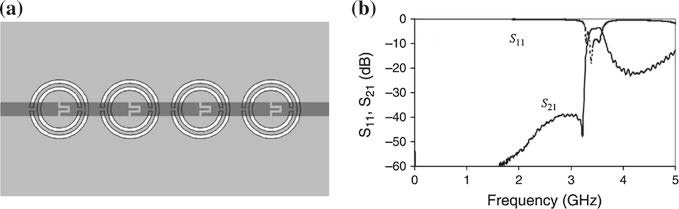
\includegraphics[width=1.0\linewidth]{sl_uvod/mstrip_csrr.jpg}
    \caption{Резонантни „леворуки`` вод на бази микрострип вода~\cite{baena}.}
    \label{uvod:sl_mstrip_csrr}
\end{figure}
Још један пример „леворуког`` вода, у микрострип технологији, приказан је на сл.~\ref{uvod:sl_mstrip_csrr}. Овде се за реализацију негативне пермитивности користи структура дуална сплит ринг резонатору, тзв. комплементарни СРР, који су ецовани у проводној равни с доње стране супстрата. Негативна пермеабилност остварена је помоћу капацитивних процепа на воду.

Водови, добијени на основу резонантног приступа, коришћени су за многе практичне примене, између осталог за развој филтара, сензора и RFID тагова~\cite{bib6,bib7,bib8}. Треба приметити да често ове примене нису директно повезане са концептом метаматеријала и ефективног хомогеног медијума. Уместо тога, фокус је на контроли дисперзије и карактеристичне импедансе на воду, као и на малој електричној величини. У том контексту, за означавање оваквих структура користе се термини као што су „водови на бази метаматеријала`` (\foreign{metamaterial-based lines}) или „водови инспирисани метаматеријалима`` (\foreign{metamaterial-inspired lines}).

%\bibliographystyle{babplai3}
%\bibliography{ref}

%\end{document}
